\documentclass[10pt,conference,compsocconf]{IEEEtran}

\usepackage{hyperref}
\usepackage{graphicx}	% For figure environment


\begin{document}
\title{Finding the Higgs boson}

\author{
  Robin Solignac,
  \textit{Department of Computer Science, EPFL Lausanne, Switzerland}\\
  Adrian Pace,
  \textit{Department of Computer Science, EPFL Lausanne, Switzerland}\\
  Yannick Schaeffer,
  \textit{Department of Computer Science, EPFL Lausanne, Switzerland}
}

\maketitle

\begin{abstract}
The Higgs boson is an elementary particle in the Standard Model of physics, which explains why other particles have mass. The Higgs boson decays rapidly into other particles and we observe the resulting signature to determine if it was a Higgs boson or some other particle / process. By using binary classification techniques, we can estimate the likelihood that a given signature was the result of a Higgs boson. This will be helpful to narrow the region where the Higgs is expected to be from the overwhelming number of noise in the dataset.
\end{abstract}

\section{Introduction}
We use binary classification techniques to estimate the likelihood that a Higgs boson is in a given snapshot of a particle collision, this data will then be used to distinguish the interesting samples that have a high probability to contain a Higgs boson from the samples where it is very likely to be only background information, mostly in the form of already known processes.

We have tried various machine learning approaches to obtain the final weights and we discuss them in section II.

In section III we compare how effective each approach we tried was, and we discuss the methodology we used to determine the best choice of parameters.

We then discuss the strength and weaknesses of our approach and conclude this paper with the implications of our method.

\section{Models and Methods}
\subsection{Background, Basic methods}
%\subsubsection{Basic methods}
\subsubsection{general\_gradient\_descent}
The general gradient descent is a function which performs the gradient descent algorithm for \emph{any} gradient and loss formula. It is simply a loop of a certain number of iterations, at each iteration we compute the gradient and move a little bit our weight vector along this gradient. Its arguments are:
\paragraph{y,tx,w} namely, the output vector, the input feature matrix and the initial weight vector from where we will start the gradient descent loop.
\paragraph{max\_iter} the number of gradient descent iterations we will do.
\paragraph{gamma} the coefficient by which will add the gradient to our current vector \(w^{t+1}=w^{t}+gamma*\nabla L(w^{t})\).
\paragraph{grad\_function} the function that will return the gradient at a given point w (y,tx,w).
\paragraph{cost\_function} the function that will return the cost at a given w (y,tx,w).


\subsubsection{general\_stochastic\_gradient\_descent}
The general stochastic gradient descent is written following the same spirit as the general gradient descent function with the main difference being it performs a stochastic gradient descend loop, meaning it only compute correction on a subset of the sample. The selection of the subset is done inside the function with the help of the batch\_iter function from the labs exercises. All arguments are the same as above, with same meaning except grad\_function is replaced by stock\_grad\_function which serve the same purpose, and there is a new batch\_size argument.
\paragraph{batch\_size} the size of the subset on which we will compute the ``partial gradient'' (the g correction term in the course notes).
\paragraph{stock\_grad\_function} the function which will compute the stochastic gradient given a subset of y, a corresponding subset of tx and the current weigth vector w.

\subsubsection{least\_squares\_GD}
Performs a general gradient descent with cost function compute\_cost\_MSE (Mean Squared Error) and gradient function compute\_gradient\_MSE, the gradient of the MSE function. Arguments have the same meaning as their homonyms described above.

\subsubsection{least\_squares\_SGD}
Performs a general stochastic gradient descent with cost function compute\_cost\_MSE (Mean Squared Error) and gradient function compute\_gradient\_MSE, the gradient of the MSE function. Arguments have the same meaning as their homonyms described above.

\subsubsection{least\_squares}
Solves directly the least square problem using linear algebra. We use, in our implementation the numpy linear system solve function to get the solution of the system presented in the course. This method provides a better accuracy and less rounding error than if we used directly the inverse formula.

\subsubsection{ridge\_regression}
We use a similar approach to the least\_squares explained above, but we introduce a regularization term in the equation controlled by the lambda\_ parameter. This adds an artificial cost proportional to the weights. Finally we solve the linear system derived in the course.

\subsubsection{logistic\_regression}
Performs logistic regression which is a gradient descent method with special cost function and associated gradient function. It is implemented by calling the general\_gradient\_descent with the new cost and gradient function.

\subsubsection{reg logistic regression}
In a similar way as the logistic regression, but with a regularization term in both the cost function and gradient function called lamdba\_. As general\_gradient\_descent only call the cost and grad function with the argument y,tx and w we need to fix the lambda\_ parameter before passing the cost and gradient function to general\_gradient\_descent. This is done using the partial function of python.

\subsection{Parameters}
There are multiple parameters in the project which can be tuned. 
\paragraph{Gamma} is the parameter describing the step of the gradient descent and of the stochastic gradient descent. At each iteration, the new weights will be calculated by adding to the current weights the derivative of the weights times gamma. It must not be too high or we will go in the direction of the good weights but miss them and go further. And at each iteration, we will further ourselves from the weights. If it is too small, we will eventually reach the best weights, but it will take a lot of time. Thus, we searched iteratively for the smallest gamma for which we got a reasonable computing time.
\begin{itemize}
\item Least square GD and Least square SGD : gamma=0.000003.
\item Logistic regression and regularized logistic regression : gamma=0.00003
\end{itemize}
\paragraph{Max iterations} this parameter describes how many steps we will take before stopping the algorithm. The higher, the more finely tuned the weights will get, and the smaller, the fastest the algorithm will be. 
\begin{itemize}
\item Least square GD and Least square SGD : max iterations=1000.
\item Logistic regression and regularized logistic regression :  max iterations=1000
\end{itemize}
\paragraph{Lambda} is the regularization parameter used to avoid over fitting. To find this parameter, we did a cross-validation (with 4 folds) and checked the test error. We tried it for 60 different lambdas between $10^{-5}$ and $10^{-2}$  \ref{fig1} for the ridge regression and between $10^{-6}$ to $10^6$ for the logistic regression. We saw that there was no lambdas for which the test error was extremely different from the train error. We can then conclude that we don’t have over fitting. This is also because we use linear models. So lambda=0.
\begin{figure}[tbp]
  \centering
  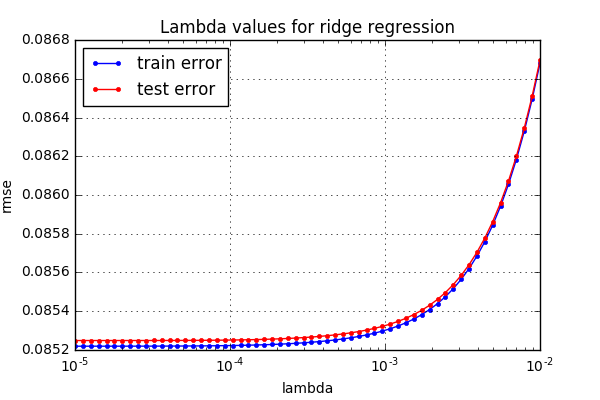
\includegraphics[width=\columnwidth]{Lambda values for ridge regression}
  \caption{Lambda effect on cleaned and normalized values for ridge regression}
  \vspace{-3mm}
  \label{fig1}
\end{figure}
\section{Final implementation}
\subsection{Data preprocessing} We have tried different preprocessing on the feature before performing machine learning on them. We tried to normalize outliers (normalizing the features of each sample when they were outside of the 95\% confidence interval of the particular feature). Furthermore we saw that a few features were at -999 so we concluded they were also outliers and we normalized them.
We also tried to rescale the data. This mean that all feature will be  mapped to \( [0,1] \) but with conservation of the relative distance between them. For each feature set we took the maximum and minimum and defined the new value x' from old value x by x' with $x' = \frac{x-\min}{\max - \min }$. This is known to improve convergence and efficacy of gradient descend algorithm, but even with this, the direct least square computation was still the most accurate function.
\subsection{Choosing the weight function} We decided to use the least square method. We chose this before the least square GD and SGD since it yielded a better mean squared error (MSE) (0.1542 and 0.1713 against 0.0852). We chose Least square over logistic regression, since when we applied the weights to the input data, classified it, and compared it to the original y, we saw that Least square was more effective than logistic regression (64695 misclassifications against 68921).
\section{Results}
With the weights obtained by our final implementation we get a success rate of $74.463\%$ on the Kaggle data set.

\section{Discussion}
Interestingly, we obtained a better estimation by computing the weights on an unnormalized data set and without removing the outliers. This might be a coincidence since the difference was minimal, but this also might mean that we are a little too narrow on our trust interval and that we accidentally removed relevant data.

Our result of $74.463\%$ may seems like a low success rate, but it has the great competitive advantage to be able to be computed very quickly since it only uses basic least square approach, thus we could easily use a far bigger training set to compute more precise weights.

On the other hand, our approach failed to try adding non linear features to our data set, and we may have missing something interesting by limiting ourselves to a linear problem.

\section{Summary}
This algorithm can be used to quickly and efficiently select a region where the Higgs boson is likely to be, and then some more expensive techniques can be implemented to look only at the region we have selected, while ignoring most of the noise. Future implementations could focus on building a computationally-heavy polynomial model around the existing weights this implementation yielded.

\bibliographystyle{IEEEtran}
\bibliography{literature}

\end{document}
